\begin{figure}
\centering
\begin{minipage}{.45\textwidth}
  \centering
  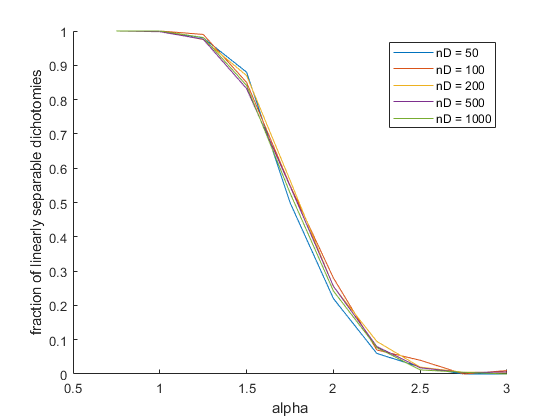
\includegraphics[width=\linewidth]{prob_ls_nD=50_1000}
  \captionof{figure}{Plots of the fraction of linearly separable dichotomies for several values of $n_D$. Here $N = 20$, $n_{max} = 100$, $c = 0$, and $\alpha = 0.75, 1, 1.25, \ldots, 3$.}
  \label{FIG:VARYND}
\end{minipage}\hspace*{.1\textwidth}%
\begin{minipage}{.45\textwidth}
  \centering
  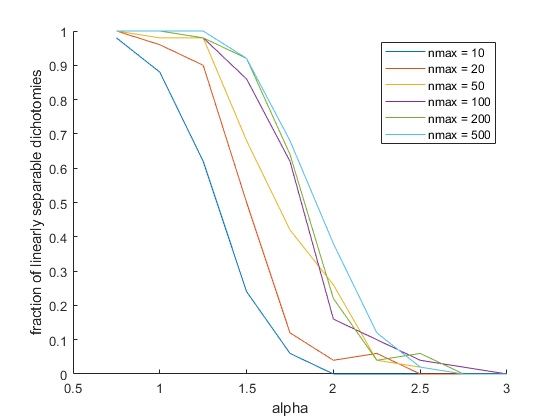
\includegraphics[width=\linewidth]{prob_ls_nmax=10_500}
  \captionof{figure}{Plots of the fraction of linearly separable dichotomies for several values of $n_{max}$. Here $N = 20$, $n_D = 50$, $c = 0$ and $\alpha = 0.75, 1, 1.25, \ldots, 3$.}
  \label{FIG:VARYNMAX}
\end{minipage}
\end{figure}

\begin{figure}
\centering
\begin{minipage}{.45\textwidth}
  \centering
  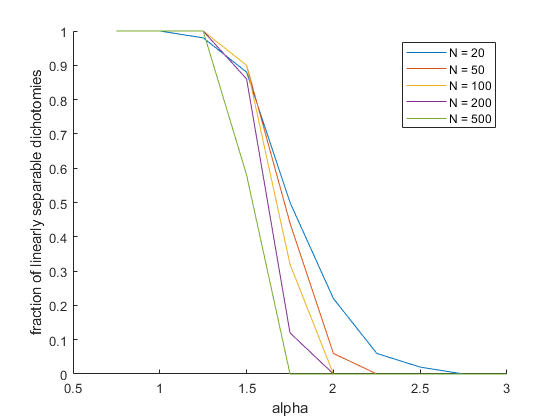
\includegraphics[width=\linewidth]{prob_ls_N=20_500}
  \captionof{figure}{Plots of the fraction of linearly separable dichotomies for several values of $N$. Here $n_{max} = 100$, $n_D = 50$, $c = 0$, and $\alpha = 0.75, 1, 1.25, \ldots, 3$.}
  \label{FIG:VARYN}
\end{minipage}\hspace*{.1\textwidth}%
\begin{minipage}{.45\textwidth}
  \centering
  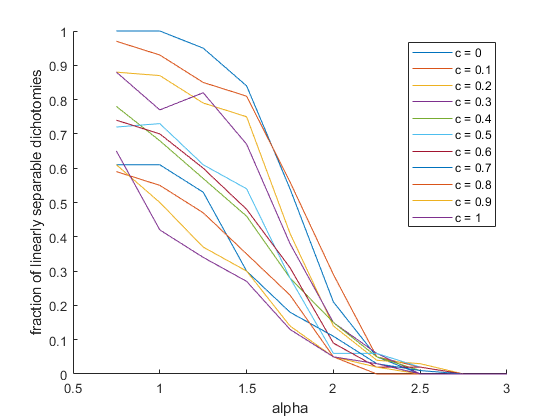
\includegraphics[width=\linewidth]{prob_ls_c=0_1(nD=100)}
  \captionof{figure}{Plots of the fraction of linearly separable dichotomies for several values of $c$. Here $N = 20$, $n_{max} = 100$ and $n_D = 100$, $c = 0$ and $\alpha = 0.75, 1, 1.25, \ldots, 3$.}
  \label{FIG:VARYC}
\end{minipage}
\end{figure}